\documentclass[10pt]{article}

\usepackage{spheric}
%%%TITLE
\title{An Enhanced ISPH-SPH Coupled Method for Incompressible Fluid-Elastic Structure Interactions}
\date{}

%%AFFILIATIONS
\author{Abbas Khayyer$^\dagger$}
\author{Hitoshi Gotoh$^*$}
\author{Yuma Shimizu}
\author{Hosein Falahaty}

\affil[]{Department of Civil and Earth Resources Engineering, Kyoto University, Kyoto, Japan}

\affil[]{\email{\dagger}{khayyer@particle.kuciv.kyoto-u.ac.jp}, \email{*}{gotoh@particle.kuciv.kyoto-u.ac.jp}}



%%DOCUMENT
\begin{document}

\maketitle

%%PLEASE PUT YOUR ABSTRACT HERE
\begin{abstract}
Precise evaluation of highly interactive fluid-structure systems (e.g. hydrodynamic slammings of marine vessels, tsunami/storm surge impact on onshore structures) has been a substantial challenge for reliable design of coastal/ocean structures. In the view of the intrinsic difficulties, usually encountered in numerical modeling of FSI (Fluid-Structure Interaction) problems associated with coastal/ocean engineering (e.g. existence of violent free-surface flows as well as large/abrupt hydrodynamic loads and consequently large structural deformations), Lagrangian meshfree methods including Smoothed Particle Hydrodynamics, SPH, are potentially robust and appropriate candidates.

In this study, a projection-based particle method, namely, Incompressible SPH (ISPH), is coupled with a SPH-based structure model in a mathematically-physically consistent manner via a careful attention to the mathematical concept of ISPH, namely, Helmholtz-Leray decomposition. The ISPH-based fluid model is founded on Navier-Stokes and continuity equations, while the SPH-based structure model is based on conservation laws for linear and angular momenta corresponding to an elastic solid. A set of previously developed enhanced schemes \cite{khayyer2017enhancement} are incorporated in the ISPH fluid model. Hence, the developed coupled method is referred to as Enhanced ISPH-SPH. \textbf{To the best of our knowledge, this study presents the first ISPH-SPH FSI solver for computational modeling of incompressible fluid flows interacting with deformable elastic structures}.

\begin{figure}[!htb]
\centering
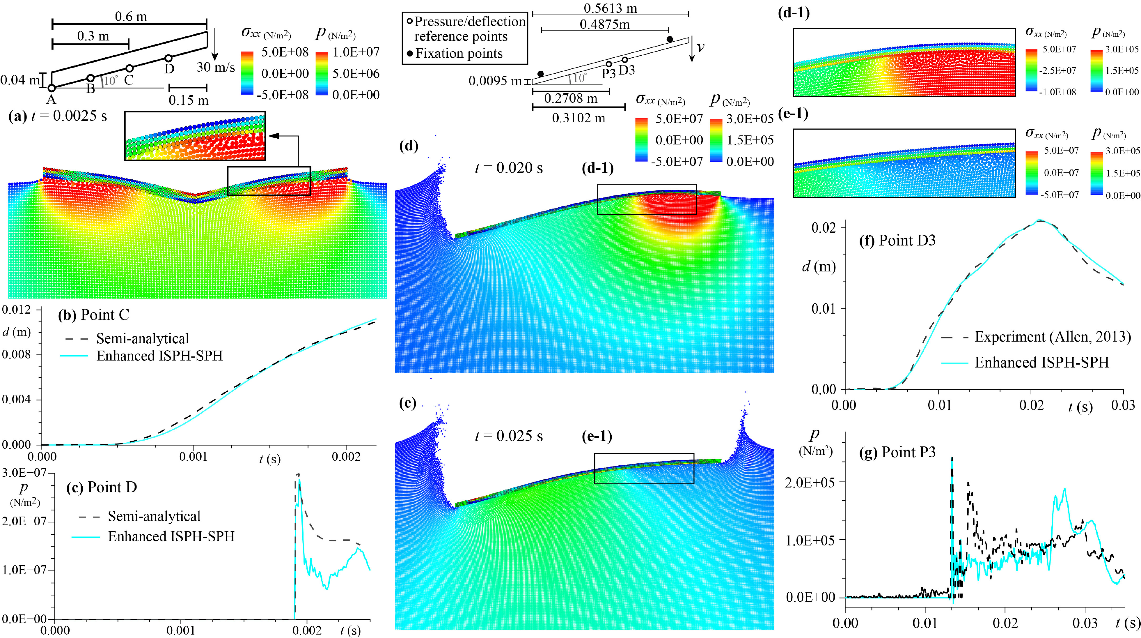
\includegraphics[width=0.95\textwidth]{2-11.png}
\caption{Representative results related to (a-c) high velocity impact of an elastic aluminum beam [2] and (d-g) hydroelastic slammings of a marine
panel \cite{allen2013mechanics,stenius2013experimental}, illustrating the performance of the developed Enhanced ISPH-SPH FSI solver}\label{fig:2}
\end{figure}

Followed by validation of the SPH structure model, the performance of Enhanced ISPH-SPH FSI solver is verified through a set of benchmark tests, namely, high velocity impact of an elastic aluminum beam \cite{oger2009simulations} and hydroelastic slammings corresponding to a marine panel \cite{allen2013mechanics,stenius2013experimental}. Fig. \ref{fig:2}(a) presents a snapshot corresponding to high velocity impact of an aluminum beam, illustrating smooth and qualitatively acceptable pressure/stress fields. Fig. \ref{fig:2}(b-c) present a quantitative validation of the accuracy of proposed FSI solver by considering the deflection and pressure time histories at two reference points. Fig. \ref{fig:2}(d-e) portray typical snapshots related to hydroelastic slammings of a marine panel (for $v = 4~\mathrm{m/s}$), illustrating qualitatively accurate pressure/stress fields. Fig. \ref{fig:2}(f-g) present quantitative validations by considering time histories of deflection and pressure at reference points D3 (for $v = 4~\mathrm{m/s}$) and P3 (for $v = 3~\mathrm{m/s}$), respectively. From the figures, the Enhanced ISPH-SPH FSI solver has provided quite accurate results corresponding to a hydroelastic slamming phenomenon.

\end{abstract}


%%THE END OF ABSTRACT

\addbib

\end{document}
